\section{Superposition von Wellen}

\textbf{Superposition beschreibt die Überlagerung (Addition) von Wellen}

\smallskip

\begin{itemize}
	\item Linearität der Wellengleichung 
	\item Die Summe zweier Lösungen der Wellengleichung ist auch eine  der Wellengleichung.
\end{itemize}

\smallskip

Das Superpositionsprinzip erlaubt die Darstellung von periodischen Wellen als eine Summe von harmonischen Wellen.


\subsection{Schwebung}

Superposition von Wellen mit \textbf{unterschiedlichen} Frequenzen \textrightarrow\  Hörbar als ein \textquotesingle Flattern\textquotesingle

$$ \boxed{f_{\text{Schwebung}} = f_2 - f_1 } $$

\begin{minipage}{0.48\columnwidth}
    $$ \xi_1 = A \cdot \sin(\omega_1 \, t) $$
\end{minipage}
\hfill
\begin{minipage}{0.48\columnwidth}
    $$ \xi_2 = A \cdot \sin(\omega_2 \, t) $$
\end{minipage}

\[
    \boxed{ \xi = 2 \, A \cdot \sin( \overline{\omega} \, t) \cdot \cos( \Omega \, t) } \qquad
    \text{mit } \overline{\omega} = \frac{\omega_1 + \omega_2}{2} \quad \text{und} \quad \Omega = \frac{\omega_2 - \omega_1}{2}
\]


\subsection{Interferenz}

Superposition von Wellen mit \textbf{gleichen} Frequenzen

\begin{minipage}[t]{0.35\columnwidth}
    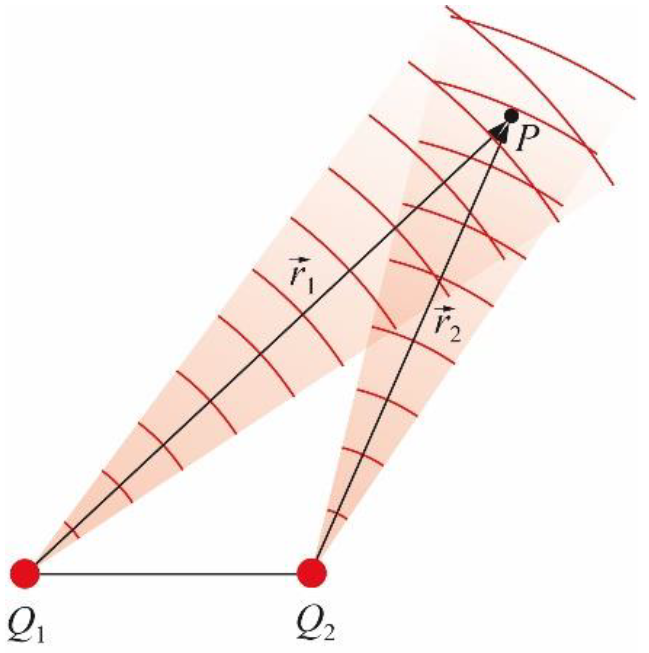
\includegraphics[width=\columnwidth, align=t]{images/interferenz.png}
\end{minipage}
\hfill
\begin{minipage}[t]{0.63\columnwidth}
    $$ \xi_1 = A \cdot \sin(\omega \, t - k \, r_1) $$
    $$ \xi_2 = A \cdot \sin(\omega \, t - k \, r_2) $$
    $$ \boxed{ \xi = 2 \, A \cdot \sin \left( \omega \, t - \frac{k (r_1 + r_2)}{2} \right) \,  \cos \left( \frac{k(r_2 - r_1)}{2}  \right) } $$

    \textrightarrow\  Der $\cos$-Term hängt nur vom Ort ab! \\
    \textrightarrow\  Es gibt \textbf{Orte}, an denen Welle sich auslöscht!
\end{minipage}



\subsection{Kohärenz}

Zwei Wellen werden als kohärent bezeichnet, wenn eine \textbf{feste Phasendifferenz} zwischen den beiden Wellen besteht.

\smallskip

\begin{outline}
    \1 Kohärenz ist eine \textbf{Vorbedingung}, damit sich eine \textbf{Interferenz} bilden kann
    \1 \textbf{Kohärenzlänge} ist der \textbf{maximale Streckenunterschied}, den zwei Wellen haben dürfen, damit eine \textbf{(stabile) Interferenz} beobachtet werden kann.
\end{outline}


\subsection{Reflexion und Transmission}

\subsubsection{Verhalten von Wellem an Grenzflächen von zwei Medien}

Ein Teil der Welle wird reflektiert und ein Teil wird transmittiert

\smallskip

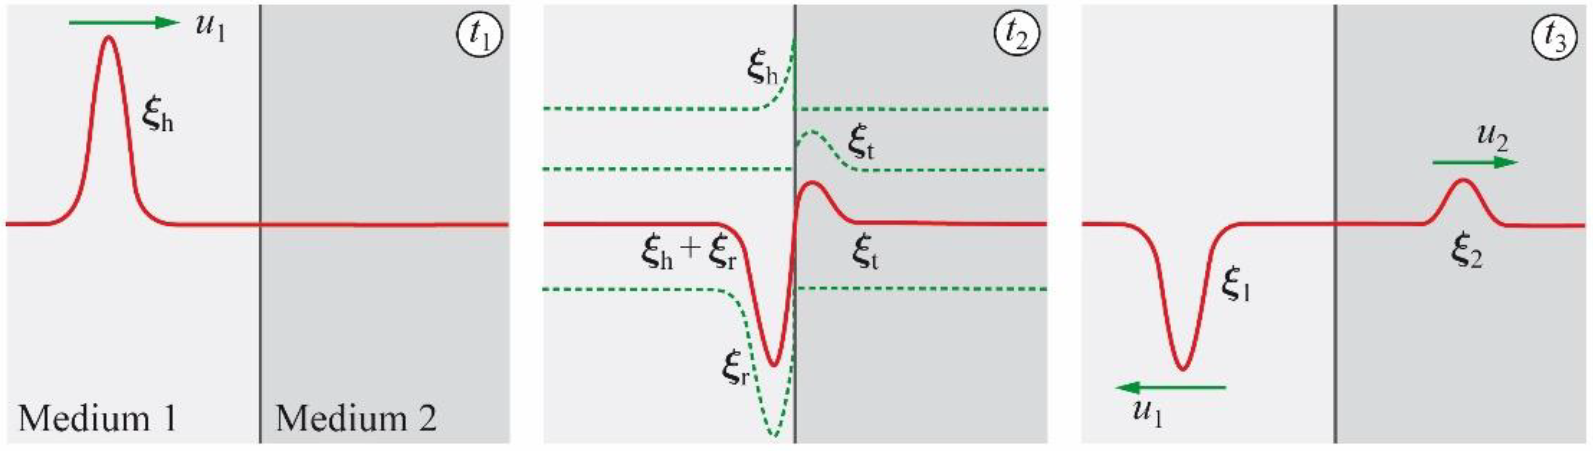
\includegraphics[width=\columnwidth]{images/reflexion_transmission.png}

\medskip
\paragraph{Physikalische Bedingung}

Stetigkeit der Wellenfunktion und der Ableitung an der Grenzfläche

$$ \xi_1(0) = \xi_2(0) \qquad \qquad \dot{\xi}_1(0) = \dot{\xi}_2(0) $$


\subsubsection{Intensität von Reflexion und Transmission}\label{Reflexion}

\begin{minipage}[t]{0.4\columnwidth}
    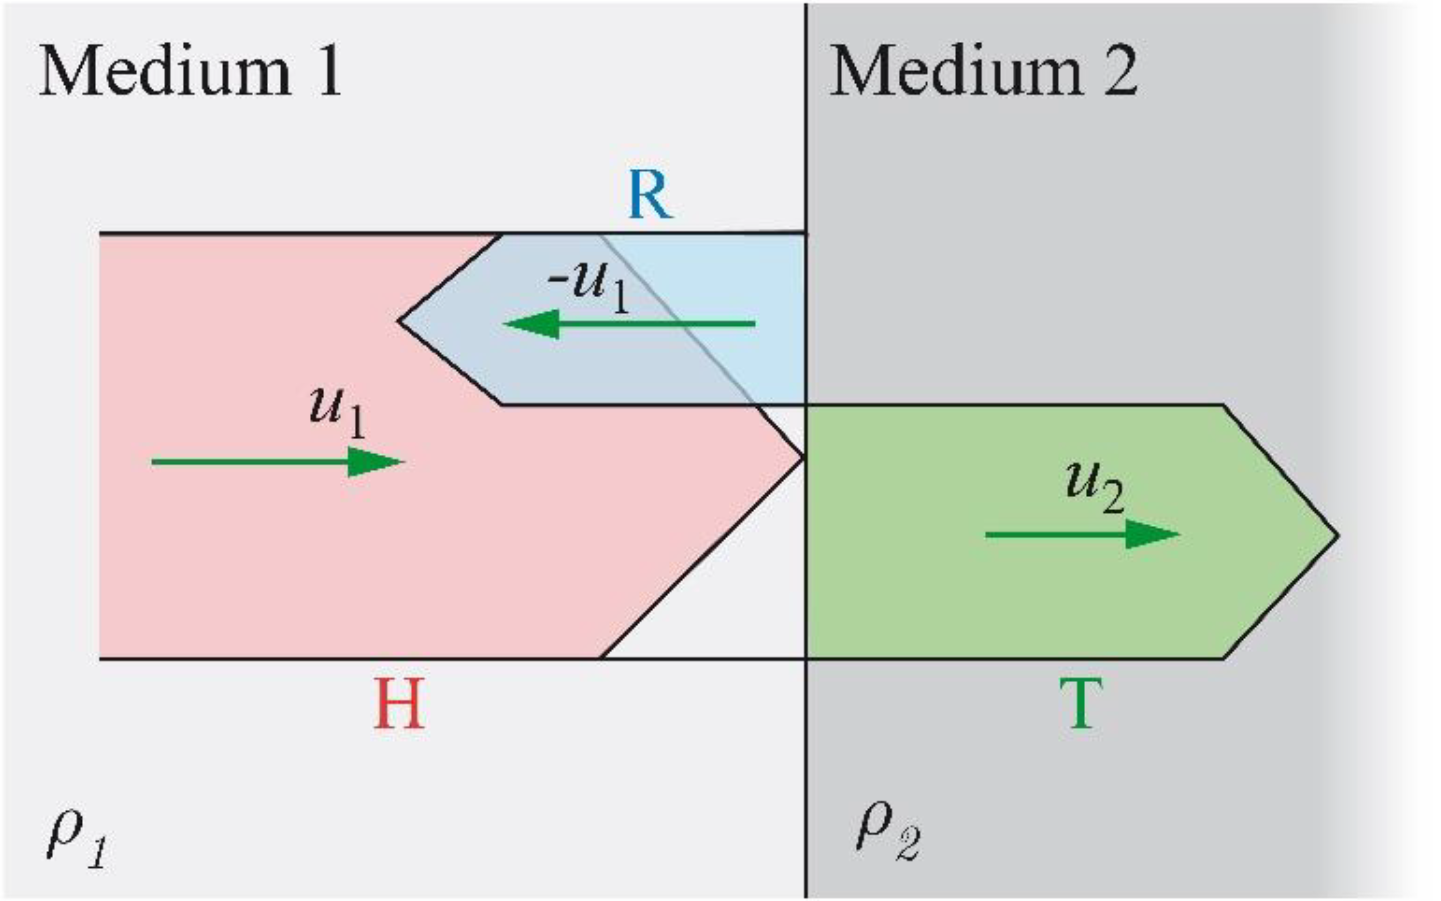
\includegraphics[width=\columnwidth, align=t]{images/reflexionskoeffizient_transmissionskoeffizient.png}
\end{minipage}
\hfill
\begin{minipage}[t]{0.58\columnwidth}
    \[ 
        \boxed{ R = \left(  \frac{Z_1 - Z_2}{Z_1 + Z_2}  \right)^2  } \qquad
        \boxed{ T = \frac{ 4 \cdot Z_1 \cdot Z_2}{(Z_1 + Z_2)^2}   }
    \]
    $$ \boxed{ \sqrt{R} = \frac{Z_1 - Z_2}{Z_1 + Z_2} = \frac{u_R}{u_H}  =\frac{A_R}{A_H} = \frac{p_R}{p_H} = \ldots } $$
    $$ \boxed{ \frac{2 \cdot Z_2}{Z_1 + Z_2} = \frac{u_T}{u_H} = \frac{A_T}{A_H} = \frac{p_T}{p_H} = \ldots } $$
\end{minipage}

\renewcommand{\arraystretch}{1.1}
\begin{ctabular}{clc}
    $R$     & Reflexionskoeffizient                 & $[R] = 1$                                                                                     \\
    $T$     & Transmissionskoeffizient              & $[T] = 1 $                                                                                    \\
    $u_H$   & Geschwindigkeit hinlaufende Welle     & $[u_H] = \frac{\meter}{\second}$                                                              \\
    $u_R$   & Geschwindigkeit reflektierte Welle    & $[u_R] = \frac{\meter}{\second}$                                                              \\
    $u_T$   & Geschwindigkeit transmittierte Welle  & $[u_T] = \frac{\meter}{\second}$                                                              \\
    $p_H$   & Druck hinlaufende Welle               & $[p_H] = \pascal$                                                                             \\
    $p_R$   & Druck reflektiert Welle               & $[p_R] = \pascal$                                                                             \\
    $p_T$   & Druck transmittierte Welle            & $[p_T] = \pascal$                                                                             \\
    $A_H$   & Amplitude hinlaufende Welle           & $[A_H] = 1$                                                                                   \\
    $A_R$   & Amplitude reflektiert Wellen          & $[A_R] = 1$                                                                                   \\
    $A_T$   & Amplitude transmittierte Welle        & $[A_T] = 1$                                                                                   \\
    $Z_i$   & Wellenwiderstand im Medium $i$        & $[Z] = \ohm = \frac{\pascal}{\meter\per\second} = \frac{\newton \, \second}{\meter\cubed}$
\end{ctabular}
\renewcommand{\arraystretch}{1}


\subsubsection{Phasensprünge bei Reflexionen}

\begin{minipage}{0.4\columnwidth}
    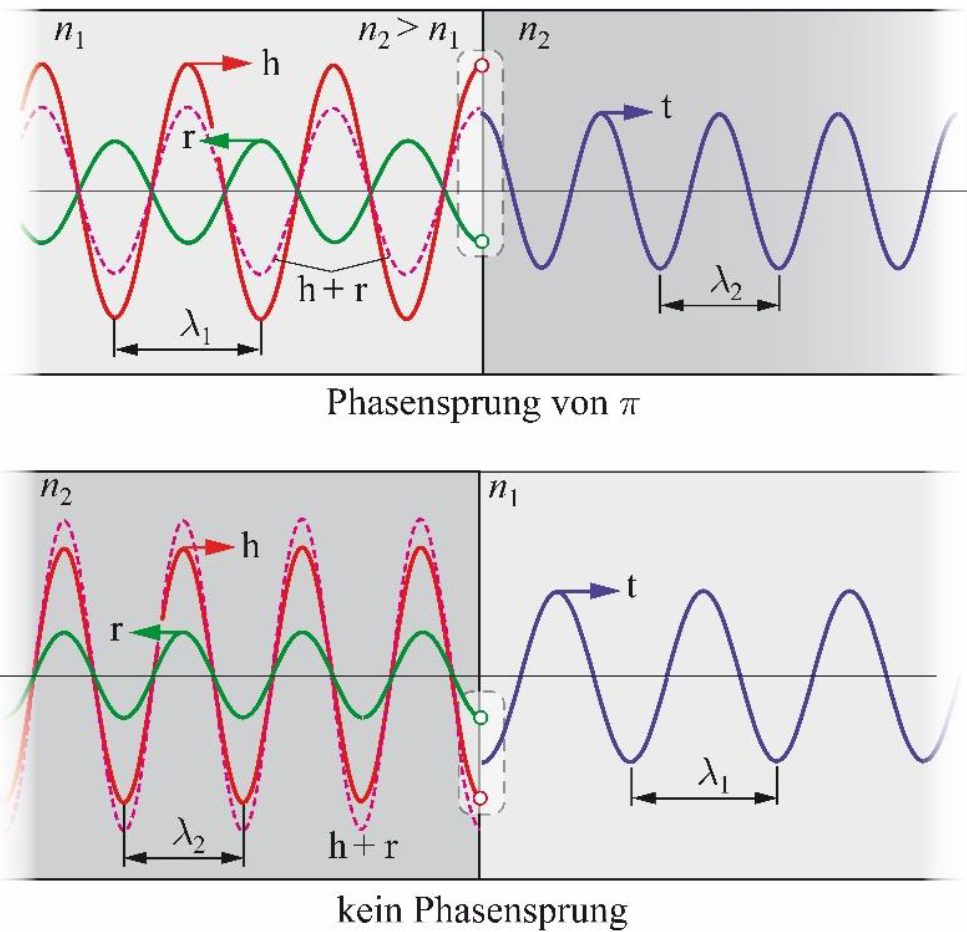
\includegraphics[width=0.9\columnwidth]{images/reflexion_phasensprung.png}
\end{minipage}
\hfill
\begin{minipage}{0.58\columnwidth}
    Reflexion an 'dichtem' Material \\
    \textrightarrow\  \textbf{Phasensprung}

    \medskip
    dicht: $n_2 > n_1$ \\
    \textbf{kleinere} Wellengeschwindigkeit, \textbf{grösserer} Wellenwiderstand

    \medskip
    Reflexion an 'dünnem' Material\\
    \textrightarrow\  \textbf{kein Phasensprung}
\end{minipage}


\subsection{Anwendung: Elektromagnetische Wellen}

\subsubsection{Elektromagnetische Wellem in Doppelleiter}

\begin{minipage}{0.48\columnwidth}
    $$ \boxed{ U_r = \frac{Z_2 - Z_1}{Z_1 + Z_2} \, U_h } $$
\end{minipage}
\hfill
\begin{minipage}{0.48\columnwidth}
    $$ \boxed{ U_t = \frac{2 \, Z_2}{Z_1 + Z_2} \, U_h } $$
\end{minipage}

\begin{minipage}{0.48\columnwidth}
    $$ \boxed{ I_r = \frac{Z_2 - Z_1}{Z_1 + Z_2} \, I_h } $$
\end{minipage}
\hfill
\begin{minipage}{0.48\columnwidth}
    $$ \boxed{ I_t = \frac{2 \, Z_1}{Z_1 + Z_2} \, I_h } $$
\end{minipage}

\medskip


\paragraph{Kabel mit kurzgeschlossenem Ende $\boldsymbol{Z_2 = 0}$}

\begin{minipage}{0.3\columnwidth}
    $$ U_r = - U_h $$
\end{minipage}
\hfill
\begin{minipage}{0.68\columnwidth}
    $$ U_1 = U_h + U_r  = U_h - U_h = 0 $$
\end{minipage}

\medskip


\paragraph{Kabel mit offenem Ende $\boldsymbol{Z_2 = \infty}$}

\begin{minipage}{0.3\columnwidth}
    $$ I_r = - I_h $$ 
\end{minipage}
\hfill
\begin{minipage}{0.68\columnwidth}
    $$ I_1 = I_r + I_h  = I_r - I_r = 0 $$  
\end{minipage}


\renewcommand{\arraystretch}{1.1}
\begin{ctabular}{clc}
    $U_r$ & Reflektierte Spannung               & $[U_r] = \volt$                                                                               \\
    $U_h$ & Eintreffende Spannung               & $[U_h] = \volt$                                                                               \\
    $I_r$ & Reflektierter Strom                 & $[I_r] = \ampere$                                                                             \\
    $I_h$ & Eintreffender Strom                 & $[I_h] = \ampere$                                                                             \\
    $Z_i$ & Wellenwiderstand im Medium $i$      & $[Z] = \ohm = \frac{\pascal}{\meter\per\second} = \frac{\newton \, \second}{\meter\cubed}$
\end{ctabular}
\renewcommand{\arraystretch}{1}


\subsubsection{Elektromagnetische Wellen in homogenem Milieu}

\[
    \boxed{ Z = \frac{E}{H} = \sqrt{ \frac{\mu_r \mu_0}{\varepsilon_r \varepsilon_0}} = \sqrt{\frac{\mu_r}{\varepsilon_r}} Z_0 = Z_0 \frac{c}{n}} \qquad 
    \boxed{ R = \left(  \frac{Z_1 - Z_2}{Z_1 + Z_2}  \right)^2 =  \left(  \frac{n_1 - n_2}{n_1 + n_2}  \right)^2 }
\]



\renewcommand{\arraystretch}{1.1}
\begin{ctabular}{clc}
    $R$             & Reflexionskoeffizient             & $[R] = 1$                                                                                     \\
    $Z_i$           & Wellenwiderstand im Medium $i$    & $[Z] = \ohm = \frac{\pascal}{\meter\per\second} = \frac{\newton \, \second}{\meter\cubed}$    \\
    $\mu_r$         & Permeabilitätszahl                & $[\mu_r] = 1$                                                                                 \\
    $\varepsilon$   & Dielektizitätszahl                & $[\varepsilon_r] = 1$                                                                         \\
    $n_i$           & Brechungsindex von Medium $i$     & $[n_1] = 1$
\end{ctabular}

\renewcommand{\arraystretch}{1.2}
\begin{ctabular}{lll}
    $\varepsilon_0$ & Ele. Feldkonstante        & $\varepsilon_0 = 8.854 \cdot 10^{-12} \, \frac{\ampere \, \second}{\volt \, \meter}$  \\
    $\mu_0$         & Magn. Feldkonstante       & $\mu_0 = 4 \pi \cdot 10^{-7} \frac{\newton}{\ampere\squared}$                         \\
    $Z_0$           & Wellenwiderstand Vakuum   & $Z_0 \approx 376.73 \, \ohm$                                                          \\
    $c$             & Lichtgeschwindigkeit      & $c = 300 \cdot 10^6 \, \frac{\meter}{\second}$
\end{ctabular}
\renewcommand{\arraystretch}{1}

\columnbreak

